\documentclass[conference]{IEEEtran}
\IEEEoverridecommandlockouts

% Standard packages supported natively on Overleaf (pdfLaTeX + BibTeX)
\usepackage{cite}
\usepackage{amsmath,amssymb,amsfonts}
\usepackage{algorithm}
\usepackage{algpseudocode}
\usepackage{graphicx}
\usepackage{textcomp}
\usepackage{xcolor}
\usepackage{booktabs}
\usepackage{array}
\usepackage{tabularx}
\usepackage{multirow}
\usepackage{tikz}
\usetikzlibrary{arrows.meta,positioning,shapes.geometric,fit,backgrounds}
\usepackage{url}
\usepackage[hidelinks]{hyperref}
\usepackage{microtype}

% Ragged-right flexible column type for clean IEEE tables
\newcolumntype{L}[1]{>{\raggedright\arraybackslash}p{#1}}
\newcolumntype{Y}{>{\raggedright\arraybackslash}X}

\def\BibTeX{{\rm B\kern-.05em{\sc i\kern-.025em b}\kern-.08em
    T\kern-.1667em\lower.7ex\hbox{E}\kern-.125emX}}

\begin{document}

\title{Multibagger Scout: A Chronologically Consistent and Verifiable Domain AI Agent for Long-Term Stock Ranking and Evidence-Grounded Financial Analysis in Taiwan}

% =========================================================================
% TODO: Fill in your author information below before submitting to Overleaf
% =========================================================================
\author{
\IEEEauthorblockN{First Author Name\textsuperscript{*}% TODO: Replace with your name
}
\IEEEauthorblockA{\textit{Department of Computer Science / Information Management}\\ % TODO: Replace with your department
\textit{University Name}\\ % TODO: Replace with your university
City, Taiwan\\ % TODO: Replace with your city
your.email@university.edu.tw} % TODO: Replace with your email
% \and
% \IEEEauthorblockN{Second Author Name}
% \IEEEauthorblockA{\textit{Department Name}\\
% \textit{University Name}\\
% City, Taiwan\\
% second.author@university.edu.tw}
}

\maketitle

\begin{abstract}
Retail participation in the Taiwan stock market reached a record 14.83 million accounts in October 2026, yet long-term shareholder wealth creation remains extremely skewed. Century-long empirical evidence (1926--2025) across 29,754 U.S. equities reveals that merely 46 firms generated half of the \$91 trillion in net wealth, with a median buy-and-hold return of $-$6.9\%; similarly, a single firm (TSMC) accounts for over 40\% of total market capitalization in Taiwan. Identifying such long-term winners \emph{ex ante} is notoriously challenging: the S\&P SPIVA 2025 scorecard reports that 79\% of active large-cap funds underperformed their benchmark and none remained in the top quartile over five consecutive years. Furthermore, quantitative backtests frequently suffer from look-ahead bias and survivorship bias---inflating cumulative returns by 30\% to 100\%---while direct application of large language models (LLMs) in financial analysis introduces pre-training temporal leakage, multi-variable arithmetic hallucinations exceeding 10\%--20\% error rates on the FAITH benchmark, and poor live trading stability (with 31 of 38 AI accounts losing money in Alpha Arena). To address these limitations, this paper proposes \textbf{Multibagger Scout}, a point-in-time (PiT), evidence-verifiable Domain AI Agent designed to evaluate the five-year potential of Taiwan Stock Exchange (TWSE) listed common stocks. Built upon an eight-module architecture inspired by the Program of Thoughts (PoT) paradigm, the system strictly decouples language reasoning from numerical computation: deterministic tools compute ten fundamental and price features alongside total wealth-preserving returns (incorporating dividends, capital reductions, and stock splits across 1,322 active and delisted firms), while an LLM planner orchestrates seven whitelisted tools (\texttt{max\_calls} $= 12$) without generating raw numbers. The primary target label (\texttt{y\_main}) identifies stocks achieving top-5\% five-year adjusted wealth returns (smoothed over a 20-trading-day terminal window) coupled with at least a 10\% five-year revenue compound annual growth rate (CAGR), explicitly retaining delisted firms and \texttt{UNKNOWN} statuses to mitigate survivorship and selection biases. For each stock query, the analytics engine integrates LightGBM ranking scores against training base rates, SHAP feature attributions, $k$-nearest neighbor ($k$NN) historical cases restricted to outcomes resolved prior to the decision date ($\tau \le t - 5\text{Y}$), and two domain red-flag rules (earnings quality and extreme valuation). A deterministic verification loop (\texttt{verify\_report}) audits all entities, dates, units, and values across up to three revision attempts before falling back to a deterministic template. Data-stage validation across eight annual rolling windows (2013--2020) is complete, covering 7,754 firm-year observations with a 0\% collection failure rate, reducing price anomaly rates from 14.7\% to 1.7\%, and achieving 8/8 external cross-check consistency. A three-round non-overlapping walk-forward evaluation protocol (2018--2020) is specified to assess ranking quality, portfolio performance versus 0050, cross-window SHAP stability, and report numerical accuracy.
\end{abstract}

\begin{IEEEkeywords}
Domain-specific AI agents, point-in-time financial analysis, multibagger stock ranking, large language models, Program of Thoughts (PoT), survivorship bias mitigation, explainable AI (SHAP), automated numerical verification.
\end{IEEEkeywords}

% =========================================================================
% SECTION I: INTRODUCTION (A-Z SOP: G, H, I, J, K, L)
% =========================================================================
\section{Introduction}

% [G. General]
Retail participation in the Taiwan equity market has reached unprecedented levels. According to Taiwan Stock Exchange (TWSE) statistics as of October 2026, cumulative retail brokerage accounts reached 14,827,469 (adding 64,000 accounts in a single month), with investors aged under 30 accounting for 56.3\% of monthly new accounts \cite{twse2026}. Despite broad retail engagement, long-term equity wealth creation exhibits extreme and intensifying right skewness. Extending global evidence across 64,000 stocks \cite{bessembinder2023}, Bessembinder's century-long empirical study of 29,754 U.S. equities from 1926 to 2025 \cite{bessembinder2026} demonstrates that although U.S. stocks generated approximately \$91 trillion in net shareholder wealth, merely 46 firms accounted for half of the total (nearly doubling in concentration relative to 89 firms in his 2018 study). Nearly 60\% of individual stocks destroyed shareholder wealth over their lifetimes, the median buy-and-hold return was $-$6.9\%, and only 41.17\% outperformed one-month Treasury bills \cite{bessembinder2026}. Taiwan displays a structurally similar concentration: Taiwan Semiconductor Manufacturing Company (TSMC) alone represents over 40\% of total TWSE market capitalization, and recent top-performing equities have clustered tightly within AI hardware supply chains \cite{twse2026}. Consequently, an open, chronologically disciplined, and evidence-verifiable research tool for evaluating five-year equity potential carries substantial practical and pedagogical value for individual investors and finance students.

% [H. However]
Translating \emph{ex post} characteristics of multi-fold winners (``multibaggers'') into reliable \emph{ex ante} screening capability, however, remains notoriously difficult. Even well-resourced institutional managers struggle to outperform consistently: the S\&P Global SPIVA Year-End 2025 Scorecard reports that 79\% of active U.S. large-cap equity funds lagged the S\&P 500, and the Persistence Scorecard reveals that 0\% of active large-cap funds remained in the top quartile across five consecutive years (2021--2025), while only 4.5\% stayed above median---worse than random chance (6.25\%) \cite{spiva2026}. Existing quantitative screening pipelines and financial AI systems suffer from four structural challenges:
\begin{enumerate}
    \item \emph{Look-Ahead and Survivorship Biases}: Backtests frequently incorporate financial statements not yet legally disclosed on the decision date or restrict the universe to currently surviving firms. Empirical audits show that survivorship bias inflates annual portfolio returns by 1--3 percentage points (30\%--100\% cumulatively over 30 years), and the open-source \texttt{pitbacktest} benchmark found that free market data sources (e.g., yfinance) correctly cover 0 of 41 prominent delisted or acquired U.S. equities \cite{gao2026}. Unadjusted cash capital reductions, stock splits, and uncleaned market-tier transitions further distort long-horizon returns.
    \item \emph{Black-Box Model Opacity}: While gradient-boosted decision trees such as LightGBM capture nonlinear cross-sectional interactions effectively \cite{gu2020}, standalone prediction scores offer neither firm-specific supporting/opposing fundamental evidence nor comparable historical precedents.
    \item \emph{LLM Pre-Training Temporal Leakage}: Recent econometric studies \cite{he2025chrono, didisheim2025, gao2026} confirm that general-purpose large language models (LLMs) memorize post-cutoff corporate outcomes embedded in pre-training corpora, causing severe look-ahead inflation when queried on historical dates.
    \item \emph{Numerical Hallucinations and Decision Instability}: Directly tasking LLMs with multi-variable financial arithmetic or autonomous trading is highly unreliable. On the FAITH benchmark (453 S\&P 500 annual reports, 2,406 numerical queries) \cite{faith2025}, frontier models incur 10\%--20\%+ error rates on multi-variable ratio calculations, while small-to-medium models approach 0\% accuracy. In live-capital testing on Nof1 Alpha Arena, 31 of 38 autonomous AI trading accounts lost money (81.6\% loss rate) \cite{alphaarena2026}, and multi-agent trading frameworks exhibit high variance across temperature and random seeds \cite{xiao2025tradingagents}.
\end{enumerate}

% [I. In Literature]
Prior research addresses facets of this problem along two primary axes. First, domain factor and empirical asset pricing studies document extreme wealth skewness \cite{bessembinder2023, bessembinder2026}, identify common traits of \emph{ex post} ten-bagger stocks such as small starting size, high book-to-market (B/M), profitability, and free cash flow (FCF) yield \cite{yartseva2025}, and demonstrate the ranking efficacy of tree-based machine learning models \cite{gu2020}. Second, financial LLM research confirms that LLMs extract statistically significant return-predictive signals from financial text \cite{lopezlira2026}, while Program of Thoughts (PoT) \cite{chen2023pot} decouples language planning from programmatic execution---eliminating 88\% of arithmetic errors in recent financial QA evaluations \cite{agenticrag2026}---and chronological consistency frameworks constrain temporal leakage \cite{he2025chrono}.

% [J. Judgement]
Despite these advances, three critical gaps remain: (i) \emph{ex post} winner profiles \cite{yartseva2025} have not been rigorously tested \emph{ex ante} across a survivorship-free Taiwan common-stock universe using non-overlapping walk-forward windows; (ii) free Taiwan equity pipelines rarely resolve cash capital reductions, loss-offsetting reductions, stock splits, and Emerging Stock Board tick-size transitions simultaneously; and (iii) existing financial agents lack a unified architecture that binds point-in-time (PiT) LightGBM, SHAP attributions, temporally resolved $k$NN cases, and domain red flags inside a whitelisted-tool verification loop guaranteeing zero unauthorized numbers.

% [K. Keypoint]
To bridge these gaps, we propose \textbf{Multibagger Scout}, a chronologically consistent and verifiable Domain AI Agent governed by a strict PoT principle: \emph{deterministic programs execute all calculations, the LLM solely selects from seven whitelisted tools and synthesizes evidence, and an automated verifier audits every reported number against tool outputs across up to three rounds before deterministic template fallback}. We define the primary target label (\texttt{y\_main}) as achieving top-5\% five-year adjusted wealth return ($\lceil 0.05 N_t \rceil$) \emph{and} a five-year revenue CAGR $\ge 10\%$, filtering out pure valuation-multiple speculation. Our study addresses three research questions:
\begin{itemize}
    \item \textbf{RQ1 (Ranking Efficacy)}: Under strict PiT April-end information constraints, do LightGBM and logistic regression outperform the $\approx$5\% base rate, 1,000 Monte Carlo random draws, single-factor screens, and an equal-weighted 0050 benchmark?
    \item \textbf{RQ2 (Feature Generalizability)}: Do ten fundamental/price features plus industry sector exhibit consistent cross-window associations (via SHAP and stratified winner/delisted analyses) when transferred to TWSE common stocks?
    \item \textbf{RQ3 (Agent Verifiability)}: Does our seven-tool PoT architecture with three-round automated verification significantly improve numerical accuracy, evidence citation rate, and required-field coverage compared to direct LLM prompting?
\end{itemize}

This work makes three contributions:
\begin{enumerate}
    \item \emph{Verified PiT Taiwan Equity Pipeline (Completed)}: We collected 1,322 TWSE common stocks (including 93 delisted firms) across 9,256 FinMind tasks with 0\% failures, implemented wealth-preserving adjustments for dividends, 280 capital-reduction firms, and 11 split firms, excluded Emerging Stock Board periods, constructed 7,754 firm-year observations (2013--2020), reduced price anomaly rates from 14.7\% to 1.7\%, and passed 8/8 external TSMC cross-checks.
    \item \emph{Non-Overlapping Walk-Forward Dual-Label Framework}: We formulate a strict three-round walk-forward protocol (2018--2020 test years) separating pure return winners (\texttt{y\_raw}) from fundamentally driven winners (\texttt{y\_main}) while honestly retaining \texttt{UNKNOWN} labels rather than coercing them to negatives.
    \item \emph{Zero-Unauthorized-Number Financial Agent}: We integrate LightGBM model scores (calibrated terminology against training base rates), SHAP explanations, temporally resolved $k$NN cases ($\tau \le t - 5\text{Y}$), two domain red-flag rules, and a three-round \texttt{verify\_report} audit loop with deterministic fallback.
\end{enumerate}

% [L. List the Organization]
The remainder of this paper is organized as follows. Section~II reviews related literature across domain factor analysis and financial AI agents and synthesizes a 4$\times$5 comparative matrix. Section~III details the Multibagger Scout architecture, PiT feature and dual-label mathematics, model tuning protocol, core algorithms, and an end-to-end TSMC case run-through. Section~IV presents completed data-stage validation results, the pending E1--E5 evaluation protocol, and key limitations. Section~V concludes and outlines future work.

% =========================================================================
% SECTION II: RELATED WORK (A-Z SOP: M, N, O)
% =========================================================================
\section{Related Work}

We organize prior work along two axes: \emph{Domain Know-How} (wealth skewness and multibagger factors) and \emph{AI Technology} (machine learning asset pricing, financial LLMs, and PoT numerical verification).

\subsection{Long-Term Wealth Skewness and Multibagger Factors}
Long-horizon stock returns follow extreme power-law skewness rather than symmetric distributions. Bessembinder et al. \cite{bessembinder2023} showed that merely 2.4\% of 64,000 global stocks accounted for all net wealth creation over 1990--2020, and Bessembinder's 100-year U.S. update (1926--2025) \cite{bessembinder2026} confirmed accelerating concentration, with 46 of 29,754 firms generating half of \$91 trillion in net wealth. Investigating 464 U.S. ten-bagger stocks over 2009--2024, Yartseva \cite{yartseva2025} identified small initial capitalization, high book-to-market ratio, positive profitability, high FCF yield, and disciplined asset growth as recurring winner traits. However, analyzing \emph{ex post} winner subsets does not establish \emph{ex ante} screening precision across a full market containing failures and delistings, nor does return sorting alone separate fundamental compounders from temporary multiple expansion.

\subsection{Machine Learning Cross-Sectional Ranking and Backtest Biases}
Gu, Kelly, and Xiu \cite{gu2020} established that tree ensembles (e.g., gradient-boosted trees) outperform linear regressions in cross-sectional return prediction by capturing nonlinear factor interactions. Yet standalone tree models remain black boxes that output opaque scores without case-level justification. Moreover, practical backtests on free data frequently suffer from survivorship bias (inflating cumulative returns by 30\%--100\% with 0/41 delisted coverage in \texttt{pitbacktest} \cite{gao2026}) and unadjusted corporate actions. In Taiwan specifically, cash capital reductions (returning par value cash while reducing share count), loss-offsetting reductions, stock splits, and concatenated Emerging-to-TWSE price histories cause severe price-anomaly contamination if unhandled.

\subsection{Financial LLMs, Multi-Agent Systems, and PoT Verification}
Lopez-Lira and Tang \cite{lopezlira2026} demonstrated in the \emph{Journal of Financial Economics} that GPT-4 headline sentiment carries statistically significant return predictability, while multi-agent systems such as TradingAgents \cite{xiao2025tradingagents} orchestrate analyst and risk-control roles. Nevertheless, recent evidence highlights three acute risks: (i) \emph{pre-training look-ahead leakage} \cite{he2025chrono, didisheim2025, gao2026}, where LLMs implicitly recall future corporate performance; (ii) \emph{multi-variable tabular hallucinations}, where FAITH \cite{faith2025} documents 10\%--20\%+ calculation error rates even for frontier models; and (iii) \emph{live trading fragility}, evidenced by 31 of 38 AI accounts losing money in Alpha Arena \cite{alphaarena2026} and reproducibility sensitivity in multi-agent trading \cite{xiao2025tradingagents}. To combat arithmetic errors, Program of Thoughts (PoT) \cite{chen2023pot} delegates numerical computation to deterministic external programs, eliminating 88\% of arithmetic errors in financial document QA \cite{agenticrag2026}.

\subsection{Novelty Positioning and 4$\times$5 Comparative Matrix}
Multibagger Scout bridges these streams by combining: (1) a survivorship-inclusive, corporate-action-adjusted TWSE PiT dataset with dual labels (\texttt{y\_main} vs. \texttt{y\_raw}) and honest \texttt{UNKNOWN} retention; (2) four-dimensional explainability (model score vs. training base rate, SHAP attributions, temporally resolved $k$NN cases with $\tau \le t - 5\text{Y}$, and two literature-backed domain red flags); and (3) a PoT agent constrained to seven whitelisted tools (\texttt{max\_calls} $= 12$) with a three-round \texttt{verify\_report} audit loop and deterministic template fallback. Table~\ref{tab:related_work} organizes the four literature streams across five evaluation dimensions.

% [O. Organize: 4x5 Literature Comparison Matrix]
\begin{table*}[t]
\centering
\caption{4$\times$5 Multi-Dimensional Literature Comparison Matrix Across Four Research Streams and Multibagger Scout Positioning}
\label{tab:related_work}
\renewcommand{\arraystretch}{1.15}
\scriptsize
\begin{tabularx}{\textwidth}{L{2.35cm} L{2.45cm} L{3.0cm} L{2.85cm} L{2.75cm} Y}
\toprule
\textbf{Literature Stream} & \textbf{Dim. 1: Representative Works \& Scope} & \textbf{Dim. 2: Core Methods \& Key Findings} & \textbf{Dim. 3: PiT Discipline \& Survivorship Control} & \textbf{Dim. 4: Numerical Reliability \& Explainability} & \textbf{Dim. 5: Multibagger Scout Breakthrough \& Trade-off} \\
\midrule
\textbf{1. Wealth Skewness \& Multibagger Factors} &
Bessembinder et al. \cite{bessembinder2023, bessembinder2026} (64k global, 29.7k U.S. 100-yr); Yartseva \cite{yartseva2025} (464 U.S. 10-baggers) &
Documents extreme wealth concentration (46 firms = 50\%); profiles size, B/M, profitability, and FCF yield traits &
\textbf{Weak (\emph{ex post} subsets)}: Infers traits from known winners without full-market \emph{ex ante} walk-forward testing &
\textbf{High intuition, low attribution}: Clear accounting logic but lacks nonlinear interaction attribution &
Extracts 10 PiT annual-report/revenue features + sector; tests \emph{ex ante} across full TWSE common stocks (incl. delisted) with revenue CAGR $\ge$10\% filter \\
\midrule
\textbf{2. ML Cross-Sectional Asset Pricing} &
Gu, Kelly \& Xiu \cite{gu2020} (U.S. asset pricing); Taiwan multi-factor ML studies &
Tree ensembles (LightGBM) and regularized linear models capture nonlinear cross-sectional interactions &
\textbf{Moderate}: Free-data pipelines often omit delisted firms (\texttt{pitbacktest}: 0/41 \cite{gao2026}) or cash capital reductions &
\textbf{Low (black box)}: Outputs scores/portfolios without firm-level pro/con evidence or historical precedents &
Covers 1,322 TWSE firms (93 delisted), adjusts dividends/reductions/splits, excludes Emerging Board (anomalies 1.7\%); adds SHAP + resolved $k$NN + 2 red flags \\
\midrule
\textbf{3. Financial LLMs \& Multi-Agent Systems} &
Lopez-Lira \& Tang \cite{lopezlira2026}; He et al. \cite{he2025chrono}; Didisheim et al. \cite{didisheim2025}; Gao et al. \cite{gao2026}; TradingAgents \cite{xiao2025tradingagents}; Alpha Arena \cite{alphaarena2026} &
Shows text-based return predictability \cite{lopezlira2026}, but raw AI trading lost money in 31/38 accounts \cite{alphaarena2026} with high seed variance \cite{xiao2025tradingagents} &
\textbf{High leakage risk}: Pre-training corpora embed post-cutoff market outcomes \cite{he2025chrono, didisheim2025, gao2026} &
\textbf{Unstable}: Unconstrained generation invites memory leakage, overtrading, and unverified claims &
Bans LLM numeric generation and external news reading; locks annual April-end feature date and restricts LLM strictly to \texttt{as\_of}=$t$ tool outputs \\
\midrule
\textbf{4. Financial Numerical Reasoning (PoT)} &
Program of Thoughts \cite{chen2023pot}; FAITH \cite{faith2025}; Agentic RAG PoT \cite{agenticrag2026} &
Quantifies 10\%--20\%+ multi-variable errors \cite{faith2025}; PoT execution eliminates 88\% of arithmetic errors \cite{agenticrag2026} &
\textbf{Neutral}: Focuses on static single-filing QA rather than multi-year walk-forward equity ranking &
\textbf{High computation accuracy}: Prevents math bugs, yet prose synthesis can still misquote units, dates, or probabilities &
Enforces 7 whitelisted tools (\texttt{max\_calls}=12) + up to 3-round \texttt{verify\_report} entity/date/unit/value audit with deterministic \texttt{template\_report($T$)} fallback \\
\bottomrule
\end{tabularx}
\end{table*}

% =========================================================================
% SECTION III: PROPOSED SYSTEM (A-Z SOP: PA-PM, [T], [PJ])
% =========================================================================
\section{Proposed System: Multibagger Scout}

\subsection{Eight-Module PoT Architecture and Design Trade-Offs}
Fig.~\ref{fig:architecture} illustrates the eight-module architecture of Multibagger Scout. Inspired by PoT \cite{chen2023pot}, Modules~(4)--(7) execute inside a deterministic Python computation sandbox, while Module~(3) (LLM Planner) orchestrates strictly seven whitelisted tools---(\texttt{analyze\_stock}, \texttt{get\_features}, \texttt{score\_model}, \texttt{find\_cases}, \texttt{check\_rules}, \texttt{follow\_up}, \texttt{verify\_report})---capped at \texttt{max\_calls} $= 12$ per user query. Every tool output is logged as a structured record containing \texttt{evidence\_id}, \texttt{stock\_id}, \texttt{as\_of}, \texttt{value}, \texttt{unit}, and \texttt{source}, aggregated into an immutable evidence bundle $T$. Module~(8a) (\texttt{verify\_report}) programmatically checks every numerical claim, entity, period, unit, and citation in draft report $R_a$ against $T$ for up to three revision attempts; if any discrepancy persists or the tool budget is exhausted, Module~(8b) returns a 100\% tool-populated deterministic \texttt{template\_report($T$)}.

% Fig. 1: Native TikZ Architecture Diagram
\begin{figure*}[t]
\centering
\resizebox{\textwidth}{!}{% Native TikZ Vector Diagram: Eight-Module PoT Architecture & 3-Round Verification Loop
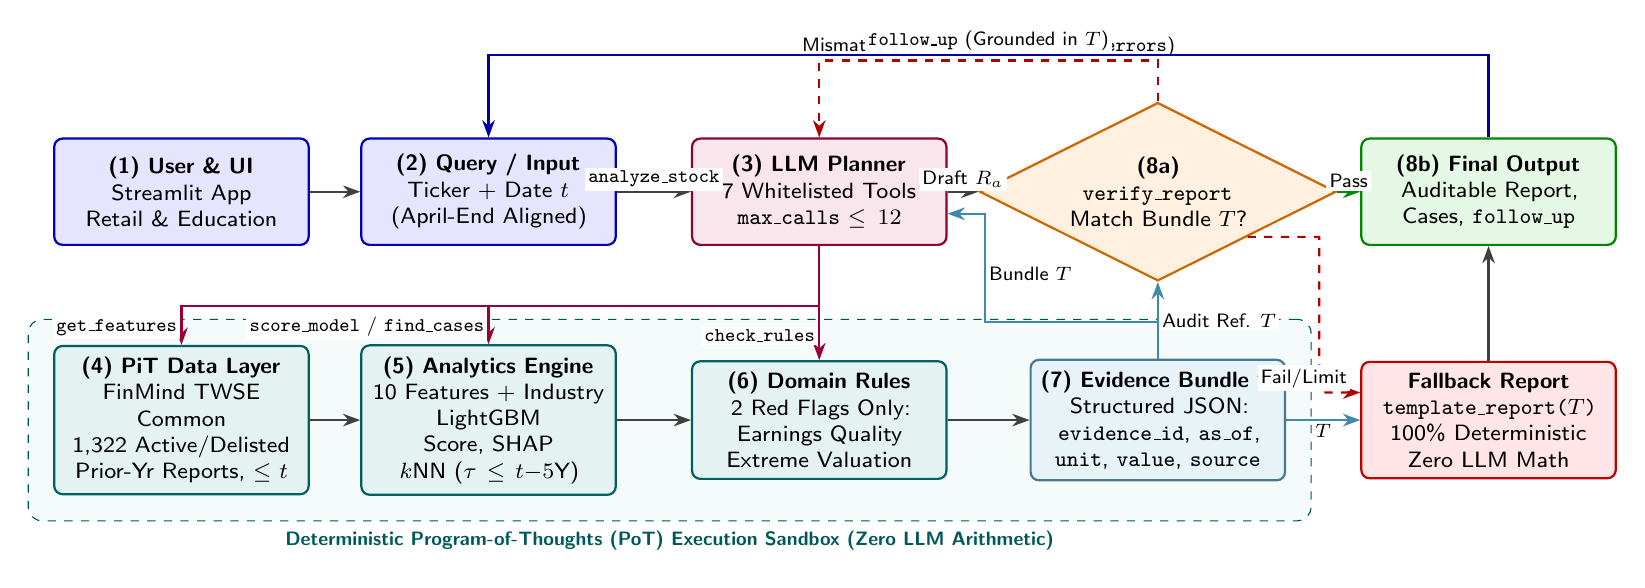
\begin{tikzpicture}[
    font=\sffamily\footnotesize,
    box/.style={
        rectangle, rounded corners=3pt, draw=#1!75!black, fill=#1!10,
        thick, align=center, minimum height=1.35cm, text width=2.95cm, inner sep=4pt
    },
    decision/.style={
        diamond, aspect=2.0, draw=orange!80!black, fill=orange!12,
        thick, align=center, inner sep=2pt, text width=2.35cm
    },
    arrow/.style={-{Stealth[length=2.2mm, width=1.6mm]}, thick, draw=black!75},
    dashedarrow/.style={-{Stealth[length=2.2mm, width=1.6mm]}, thick, dashed, draw=red!70!black},
    lbl/.style={font=\sffamily\scriptsize, fill=white, inner sep=1.2pt}
]

% Row 1: Top Orchestration & Verification Layer (y = 0)
\node[box=blue] at (0, 0) (user) {\textbf{(1) User \& UI}\\Streamlit App\\Retail \& Education};
\node[box=blue] at (3.9, 0) (query) {\textbf{(2) Query / Input}\\Ticker + Date $t$\\(April-End Aligned)};
\node[box=purple] at (8.1, 0) (planner) {\textbf{(3) LLM Planner}\\7 Whitelisted Tools\\\texttt{max\_calls} $\le 12$};
\node[decision] at (12.4, 0) (verify) {\textbf{(8a) \texttt{verify\_report}}\\Match Bundle $T$?};
\node[box=green!70!black] at (16.6, 0) (output) {\textbf{(8b) Final Output}\\Auditable Report,\\Cases, \texttt{follow\_up}};

% Row 2: Deterministic PoT Layer & Fallback (y = -2.9)
\node[box=teal] at (0, -2.9) (data) {\textbf{(4) PiT Data Layer}\\FinMind TWSE Common\\1,322 Active/Delisted\\Prior-Yr Reports, $\le t$};
\node[box=teal] at (3.9, -2.9) (analytics) {\textbf{(5) Analytics Engine}\\10 Features + Industry\\LightGBM Score, SHAP\\$k$NN ($\tau \le t{-}5\text{Y}$)};
\node[box=teal] at (8.1, -2.9) (domain) {\textbf{(6) Domain Rules}\\2 Red Flags Only:\\Earnings Quality\\Extreme Valuation};
\node[box=cyan!70!black] at (12.4, -2.9) (bundle) {\textbf{(7) Evidence Bundle $T$}\\Structured JSON:\\\texttt{evidence\_id}, \texttt{as\_of},\\\texttt{unit}, \texttt{value}, \texttt{source}};
\node[box=red] at (16.6, -2.9) (fallback) {\textbf{Fallback Report}\\\texttt{template\_report($T$)}\\100\% Deterministic\\Zero LLM Math};

% Background frame for Deterministic PoT Execution Sandbox
\begin{scope}[on background layer]
    \node[rectangle, rounded corners=5pt, draw=teal!65!black, dashed, fill=teal!4,
          inner sep=9pt, fit=(data)(analytics)(domain)(bundle),
          label={[font=\sffamily\scriptsize\bfseries, text=teal!70!black]south:Deterministic Program-of-Thoughts (PoT) Execution Sandbox (Zero LLM Arithmetic)}] {};
\end{scope}

% Top Row Main Flow
\draw[arrow] (user.east) -- (query.west);
\draw[arrow] (query.east) -- node[lbl, above]{\texttt{analyze\_stock}} (planner.west);
\draw[arrow] (planner.east) -- node[lbl, above]{Draft $R_a$} (verify.west);
\draw[arrow, draw=green!55!black] (verify.east) -- node[lbl, above]{Pass} (output.west);

% Tool Invocations from Planner down to Sandbox (clean horizontal bus at y = -1.45)
\draw[arrow, draw=purple!80!black] (planner.south) -- (8.1, -1.45) -- (0, -1.45) -- node[lbl, pos=0.55, left]{\texttt{get\_features}} (data.north);
\draw[arrow, draw=purple!80!black] (3.9, -1.45) -- node[lbl, pos=0.55, left]{\texttt{score\_model} / \texttt{find\_cases}} (analytics.north);
\draw[arrow, draw=purple!80!black] (8.1, -1.45) -- node[lbl, pos=0.55, left]{\texttt{check\_rules}} (domain.north);

% Deterministic Sandbox Dataflow (Left to Right)
\draw[arrow] (data.east) -- (analytics.west);
\draw[arrow] (analytics.east) -- (domain.west);
\draw[arrow] (domain.east) -- (bundle.west);

% Evidence Bundle T feeds Verifier and Planner (routed in clean channel x=10.2)
\draw[arrow, draw=cyan!65!black] (bundle.north) -- node[lbl, right]{Audit Ref. $T$} (verify.south);
\draw[arrow, draw=cyan!65!black] (12.4, -1.65) -- (10.2, -1.65) |- ([yshift=-0.28cm]planner.east) node[lbl, pos=0.22, right]{Bundle $T$};

% Retry Loop (above Row 1)
\draw[dashedarrow] (verify.north) -- ++(0, 0.52) -| node[lbl, pos=0.25, above]{Mismatch \& attempt $< 3$ (Return \texttt{errors})} (planner.north);

% Follow-up Loop (higher above Row 1)
\draw[arrow, draw=blue!65!black] (output.north) -- ++(0, 1.05) -| node[lbl, pos=0.25, above]{\texttt{follow\_up} (Grounded in $T$)} (query.north);

% Fallback Path on Exhaustion (routed in clean channel x=14.45 between bundle and fallback)
\draw[dashedarrow] (verify.south east) -| (14.45, -2.55) -- ([yshift=0.35cm]fallback.west) node[lbl, pos=0.2, above, xshift=-0.3cm]{Fail/Limit};
\draw[arrow, draw=cyan!65!black] (bundle.east) -- node[lbl, below]{$T$} (fallback.west);
\draw[arrow] (fallback.north) -- (output.south);

\end{tikzpicture}
}
\caption{Eight-module Program-of-Thoughts (PoT) architecture of Multibagger Scout. All numerical computations occur inside the deterministic sandbox (Modules~4--7) via seven whitelisted tools (\texttt{max\_calls} $\le 12$), and every draft report undergoes up to three rounds of automated \texttt{verify\_report} auditing before deterministic \texttt{template\_report($T$)} fallback.}
\label{fig:architecture}
\end{figure*}

This architecture codifies three explicit engineering trade-offs:
\begin{enumerate}
    \item \emph{Temporal Granularity vs. Zero Look-Ahead}: Fixing the annual feature date $t_y$ to the last trading day of April and utilizing only prior-year annual reports (Dec~31, legally filed by March~31) and prior-year Jan--Dec monthly revenues (disclosed by Jan~10) sacrifices up to 16 months of feature recency (deferring quarterly filings to future work) in exchange for 100\% verifiable chronological consistency without paid restatement timestamps.
    \item \emph{Agent Freedom vs. Zero Numerical Hallucination}: Restricting the LLM to seven pre-verified tools and prohibiting external news reading or arbitrary code synthesis trades open-ended flexibility for guaranteed traceability of every reported number.
    \item \emph{Sample Size vs. Label Purity}: Limiting the universe to TWSE-listed common stocks and assigning indeterminate delistings or price anomalies to \texttt{UNKNOWN} reduces sample count but prevents conflating M\&A buyouts or data discontinuities with business failures.
\end{enumerate}

\subsection{Point-in-Time Universe and Fixed 10-Feature Specification}
At each annual feature date $t_y$ (last trading day of April for year $y \in \{2013,\dots,2020\}$), the eligible universe $\mathcal{U}_{t_y}$ includes only TWSE-listed common stocks (4-digit tickers not starting with \texttt{0}, explicitly retaining subsequently delisted firms; excluding \texttt{9}-prefix TDRs, ETFs, preferred shares, and TPEx/OTC listings) that have been listed for at least one full year and are not in the bottom 10\% of prior-year average daily trading value. Because FinMind concatenates pre-listing Emerging Stock Board quotes with TWSE quotes, we automatically detect and exclude any firm-year with $\ge 5$ trading days in the 90 days preceding $t_y$ whose OHLC prices violate official TWSE tick-size increments.

Table~\ref{tab:features} specifies the fixed set of 10 numerical features plus Industry Category computed strictly from year $y-1$ disclosures and prices $\le t_y$. Five candidate metrics removed during specification pruning (ROA, EBITDA margin, asset growth rate, return volatility, and dividend yield) are strictly excluded to maintain parsimony and avoid feature creep.

\begin{table}[t]
\centering
\caption{Fixed Point-in-Time Feature Set (10 Metrics + Industry Category) Computed at April-End Feature Date $t_y$}
\label{tab:features}
\renewcommand{\arraystretch}{1.12}
\scriptsize
\begin{tabularx}{\columnwidth}{c L{2.25cm} Y}
\toprule
\textbf{\#} & \textbf{Feature Name} & \textbf{Strict Point-in-Time Definition ($\le t_y$)} \\
\midrule
1 & Market Capitalization & Closing price at $t_y \times (\text{Paid-in Capital}_{y-1} / 10) \times k$ (capital-reduction share-ratio adjusted) \\
2 & FCF Yield & $(\text{OCF}_{y-1} - \text{CapEx}_{y-1}) / \text{Market Cap}_{t_y}$ \\
3 & Book-to-Market (B/M) & $\text{Total Equity}_{y-1} / \text{Market Cap}_{t_y}$ \\
4 & Price-to-Earnings (P/E) & FinMind TWSE PER as of $t_y$ (year $y-1$ earnings basis) \\
5 & ROE & $\text{Net Income}_{y-1} / \text{Average Equity}_{y-1}$ \\
6 & Gross Margin & $\text{Gross Profit}_{y-1} / \text{Revenue}_{y-1}$ \\
7 & Annual Revenue Growth & $(\text{Rev}_{y-1} - \text{Rev}_{y-2}) / \text{Rev}_{y-2}$ (Jan--Dec sums) \\
8 & OCF / Net Income & $\text{Operating Cash Flow}_{y-1} / \text{Net Income}_{y-1}$ \\
9 & Debt Ratio & $\text{Total Liabilities}_{y-1} / \text{Total Assets}_{y-1}$ \\
10 & Trailing 12M Return & 12-month adjusted wealth return ending at $t_y$ \\
$+$ & Industry Category & Official TWSE sector classification (categorical) \\
\bottomrule
\end{tabularx}
\end{table}

\subsection{Formal Mathematical Definitions: Adjusted Wealth, Dual Labels, and Walk-Forward Isolation}
Let $P_{i,t}$ denote the closing price of stock $i$ on April-end feature date $t$. For any subsequent trading day $d > t$, let $\mathcal{E}_{i,(t,d]}$ be the set of corporate actions (cash/stock dividends, capital reduction trading resumptions, and stock splits/par-value changes) occurring in $(t, d]$. Denoting the pre-event closing price by $P_{i,e^-}^{\text{close}}$ and the TWSE-announced reference price by $P_{i,e}^{\text{ref}}$, the wealth-preserving factor $f_e$ and cumulative adjusted wealth sequence $W_{i, t \to d}$ are defined as:
\begin{equation}
\label{eq:wealth}
f_e = \frac{P_{i, e^-}^{\text{close}}}{P_{i, e}^{\text{ref}}}, \qquad W_{i, t \to d} = \frac{P_{i,d}}{P_{i,t}} \prod_{e \in \mathcal{E}_{i,(t,d]}} f_e.
\end{equation}

To prevent terminal single-day price spikes from distorting five-year outcomes, let $\mathcal{V}_{i, t+5}$ denote the final $M = 20$ trading days ending at the five-year horizon $t + 5\text{Y}$ (with 5-day and 60-day horizons reserved for sensitivity analysis E5). The five-year adjusted wealth return $r_{i,t}$ is:
\begin{equation}
\label{eq:return}
r_{i,t} = \left( \frac{1}{20} \sum_{d \in \mathcal{V}_{i, t+5}} W_{i, t \to d} \right) - 1.
\end{equation}

When a capital reduction occurs between fiscal year-end (Dec~31) and feature date $t$, the post-to-pre share-count ratio $k$ required for accurate Market Capitalization is recovered from official event prices as:
\begin{equation}
\label{eq:ratio_k}
k = \begin{cases}
\dfrac{P_{i,e^-}^{\text{close}}}{P_{i,e}^{\text{ref}}}, & \text{loss-offsetting reduction}, \\[9pt]
\dfrac{P_{i,e^-}^{\text{close}} - 10}{P_{i,e}^{\text{ref}} - 10}, & \text{cash capital reduction (NT\$10 par)}.
\end{cases}
\end{equation}

Two conservative data-hygiene filters are enforced: (i) any stock exhibiting a post-adjustment single-day wealth change exceeding TWSE daily price limits (7\% prior to June~2015, 10\% thereafter) is flagged as a \emph{price anomaly}; (ii) any revenue jumping $> 3\times$ across the 2012$\to$2013 IFRS transition (e.g., 2605 Sincere Navigation jumping 31.8$\times$ due to subsidiary consolidation) is marked missing. Let $\mathcal{U}_t^{\text{rank}} \subseteq \mathcal{U}_t$ be the anomaly-free rankable universe of size $N_t = |\mathcal{U}_t^{\text{rank}}|$, and let $\mathcal{W}_t$ be the top $K_t = \lceil 0.05 N_t \rceil$ stocks ranked by $r_{i,t}$ (ties broken by ascending ticker). With five-year revenue CAGR $g_{i,y} = (\text{Rev}_{i, y+4} / \text{Rev}_{i, y-1})^{1/5} - 1$, the control label $y_{\text{raw}}(i,t)$ and primary label $y_{\text{main}}(i,t)$ are formally defined as:
\begin{equation}
\label{eq:yraw}
y_{\text{raw}}(i,t) = \begin{cases}
1, & i \in \mathcal{W}_t, \\
0, & i \in \mathcal{U}_t^{\text{rank}} \setminus \mathcal{W}_t, \\
\text{UNKNOWN}, & i \notin \mathcal{U}_t^{\text{rank}},
\end{cases}
\end{equation}
\begin{equation}
\label{eq:ymain}
y_{\text{main}}(i,t) = \begin{cases}
1, & y_{\text{raw}}=1 \wedge g_{i,y}\text{ valid} \wedge g_{i,y} \ge 0.10, \\
0, & y_{\text{raw}}=0 \vee (y_{\text{raw}}=1 \wedge g_{i,y}\text{ valid} \wedge g_{i,y} < 0.10), \\
\text{UNKNOWN}, & y_{\text{raw}}=\text{UNKNOWN} \vee (y_{\text{raw}}=1 \wedge g_{i,y}\text{ invalid}).
\end{cases}
\end{equation}
Crucially, \texttt{UNKNOWN} instances (price anomalies, IFRS discontinuities, or firms delisted before year $y+4$) are \emph{never} coerced to negative ($0$); they are excluded from model training and primary evaluation and transparently disclosed per round.

Let $\mathbf{x}_{i,t_y}$ be the feature vector derived strictly from public information $\mathcal{I}_{i,t_y}$ available on or before $t_y$, and let $a_{i,y} = t_y + 5\text{Y}$ denote the exact timestamp when all inputs needed to resolve $y_{\text{main}}(i, t_y)$ become public. For each walk-forward round $k \in \{1, 2, 3\}$ with test feature date $t_{\text{test}}^{(k)} \in \{\text{2018-04}, \text{2019-04}, \text{2020-04}\}$, the training set $\mathcal{D}_{\text{train}}^{(k)}$ and retrievable $k$NN historical case pool $\mathcal{C}^{(k)}$ obey strict non-overlapping temporal isolation:
\begin{equation}
\label{eq:walkforward}
\mathcal{D}_{\text{train}}^{(k)} = \mathcal{C}^{(k)} = \left\{ \big(\mathbf{x}_{i,t_y}, y_{\text{main}}(i,t_y)\big) \;\middle|\; a_{i,y} \le t_{\text{test}}^{(k)} \wedge y_{\text{main}} \in \{0,1\} \right\}.
\end{equation}
All imputers, scalers, encoders, and domain rule quantile thresholds $\theta_{\text{train}}^{(k)}$ are fitted exclusively on $\mathcal{D}_{\text{train}}^{(k)}$ and applied unchanged to $\mathcal{D}_{\text{test}}^{(k)}$.

\subsection{Analytics Engine, Domain Red Flags, and Hyperparameter Protocol}
Module~(5) pairs LightGBM (primary ranker) with L2-regularized Logistic Regression (baseline) under a fixed random seed (\texttt{SEED} $= 42$). Prior to probability calibration, raw model outputs are strictly termed \textbf{model scores} (never ``upside probabilities''), and we maintain a clear separation between the \emph{report comparison benchmark} (training-period positive rate of \texttt{y\_main}) and the \emph{E1 evaluation benchmark} (in-round actual test positive rate). SHAP values quantify each feature's positive or negative push, while Euclidean $k$NN retrieves the top-$k$ closest resolved positive (\texttt{y\_main} $= 1$) and negative (\texttt{y\_main} $= 0$) historical cases from $\mathcal{C}^{(k)}$ ($\tau \le t - 5\text{Y}$).

Module~(6) enforces exactly two deterministic domain red-flag rules backed by static literature annotations in \texttt{knowledge/} (no external news scraping or dynamic RAG):
\begin{enumerate}
    \item \emph{Earnings Quality Red Flag}: Triggered when OCF/Net Income falls below the training-window lower quantile threshold, signaling potential accrual-driven earnings fragility.
    \item \emph{Extreme Valuation Red Flag}: Triggered when P/E or B/M falls into the extreme overvaluation tail of the training distribution, warning against multiple-compression risk.
\end{enumerate}

To prevent test-set overfitting, hyperparameters are strictly locked during testing and tuned solely within the training period (Table~\ref{tab:tuning}).

% [T] Hyperparameter Tuning Table
\begin{table*}[t]
\centering
\caption{Model Hyperparameter Defaults and In-Training Tuning Space (Fixed \texttt{SEED} $= 42$, Strictly Locked During Test Windows)}
\label{tab:tuning}
\renewcommand{\arraystretch}{1.12}
\scriptsize
\begin{tabularx}{\textwidth}{L{2.3cm} L{2.6cm} L{3.1cm} L{3.6cm} Y}
\toprule
\textbf{Model / Component} & \textbf{Hyperparameters} & \textbf{Fixed Default (Small Train Set)} & \textbf{In-Training Search Space ($\ge$2 Train Yrs, PR-AUC)} & \textbf{Anti-Overfitting Design Rationale} \\
\midrule
\textbf{LightGBM} & \texttt{max\_depth}, \texttt{num\_leaves} & \texttt{max\_depth}$=3$, \texttt{num\_leaves}$=7$ & \texttt{max\_depth} $\in \{3, 4\}$, \texttt{num\_leaves} $\in \{7, 15\}$ & Shallow trees prevent memorizing single-year noise across 10 features + sector \\
\textbf{LightGBM} & \texttt{learning\_rate}, \texttt{n\_estimators} & \texttt{lr}$=0.05$, \texttt{n\_estimators}$=100$ & \texttt{lr} $\in \{0.03, 0.05\}$, \texttt{n\_estimators} $\in \{100, 200\}$ & Paired with \texttt{min\_child\_samples} $\in \{20, 50\}$ and \texttt{colsample\_bytree}$=0.8$ \\
\textbf{LightGBM} & \texttt{class\_weight} & \texttt{'balanced'} & \texttt{'balanced'} (auto-scaled per round) & Addresses severe class imbalance ($\le 5\%$ positive rate in \texttt{y\_main}) \\
\textbf{Logistic Reg.} & Regularization, weight & \texttt{penalty='l2'}, $C=1.0$, \texttt{'balanced'} & $C \in \{0.1, 1.0, 10.0\}$ & Median imputation + Z-score scaling fitted solely on $\mathcal{D}_{\text{train}}^{(k)}$ \\
\textbf{$k$NN Cases} & Neighbors $k$, metric & $k=3$ (3 pos. + 3 neg.), Euclidean & $k \in \{3, 5\}$ & Standardized on $\mathcal{D}_{\text{train}}^{(k)}$; strictly queries \texttt{label\_available\_by} $\le t$ \\
\bottomrule
\end{tabularx}
\end{table*}

\subsection{Core Algorithms and End-to-End TSMC Case Run-Through}
Algorithms~\ref{alg:agent} and~\ref{alg:dataset} formalize the PoT agent orchestration with three-round numerical verification and the PiT dual-label dataset construction pipeline, respectively.

% Algorithm 1: Agent Main Execution & 3-Round Verification Loop
\begin{algorithm}[t]
\caption{Multibagger Scout Agent \& 3-Round Verification}
\label{alg:agent}
\scriptsize
\begin{algorithmic}[1]
\Require User query $q$, stock ticker $s$, analysis date $d$, budget $B_{\max}{=}12$
\Ensure Verified report $R^*$ (or deterministic fallback)
\State $(intent, t, eligible) \gets \texttt{analyze\_stock}(s, d)$ \Comment{Align $t$ to April-end}
\If{\textbf{not} $eligible$}
    \State \Return \texttt{limited\_report}($s, t$, ``Ineligible universe or date'')
\EndIf
\State $calls \gets 1$;\; $E \gets \texttt{get\_features}(s, \text{as\_of}{=}t)$;\; $calls \gets calls + 1$
\State $(score, tier, base, shap) \gets \texttt{score\_model}(E, t)$;\; $calls \gets calls + 1$
\State $cases \gets \texttt{find\_cases}(E, \text{label\_available\_by}{=}t)$;\; $calls \gets calls + 1$
\State $flags \gets \texttt{check\_rules}(E, \theta_{\text{train}}(t))$;\; $calls \gets calls + 1$
\State $T \gets \texttt{evidence\_bundle}(E, score, tier, base, shap, cases, flags)$
\State $ctx \gets \emptyset$
\For{$attempt = 1$ \textbf{to} $3$}
    \If{$calls \ge B_{\max}$} \textbf{break} \EndIf
    \State $R_a \gets \texttt{LLM\_synthesize}(q, T, ctx)$ \Comment{Zero raw math by LLM}
    \State $errors \gets \texttt{verify\_report}(R_a, T)$;\; $calls \gets calls + 1$
    \If{$errors = \emptyset$}
        \State \Return $R_a$ \Comment{All entities, dates, units, values verified}
    \EndIf
    \State $ctx \gets ctx \cup errors$ \Comment{Feed discrepancies for rewrite}
\EndFor
\State \Return \texttt{template\_report}($T$) \Comment{100\% deterministic fallback}
\end{algorithmic}
\end{algorithm}

% Algorithm 2: Point-in-Time Dataset & Dual-Label Construction
\begin{algorithm}[t]
\caption{Point-in-Time Dataset \& Dual-Label Builder}
\label{alg:dataset}
\scriptsize
\begin{algorithmic}[1]
\Require TWSE active + delisted pool (1,322 firms), years $Y{=}\{2013,\dots,2020\}$
\Ensure Point-in-Time dataset $\mathcal{D}$ with \texttt{y\_raw}, \texttt{y\_main}, \texttt{UNKNOWN}
\State $\mathcal{D} \gets \emptyset$
\For{each year $y \in Y$}
    \State $t_y \gets$ last TWSE trading day of April in year $y$
    \State Filter listed $\ge 1$ yr, drop bottom 10\% prior-yr turnover, drop Emerging Board ($\ge 5$ off-tick days in 90d) $\rightarrow \mathcal{U}_{t_y}$
    \For{each stock $i \in \mathcal{U}_{t_y}$}
        \State Compute 10 features $\mathbf{x}_{i,t_y}$ using year $y{-}1$ reports, $y{-}1$ revenues, $\le t_y$ prices, and ratio $k$ via Eq.~(\ref{eq:ratio_k})
        \State Build $W_{i,t_y \to d}$ via Eq.~(\ref{eq:wealth}); check 7\%/10\% daily limit anomalies
        \State If anomaly-free, compute 20-day mean $r_{i,t_y}$ via Eq.~(\ref{eq:return})
    \EndFor
    \State Rank $\mathcal{U}_{t_y}^{\text{rank}}$ ($N_t$ firms); select top $K_t = \lceil 0.05 N_t \rceil \rightarrow \mathcal{W}_{t_y}$
    \For{each stock $i \in \mathcal{U}_{t_y}$}
        \State Check 2012$\to$2013 IFRS jump ($>3\times$) and 5-yr survival for $g_{i,y}$
        \State Assign $y_{\text{raw}}(i,t_y)$ and $y_{\text{main}}(i,t_y)$ via Eqs.~(\ref{eq:yraw})--(\ref{eq:ymain})
        \State $\mathcal{D} \gets \mathcal{D} \cup \{(\mathbf{x}_{i,t_y}, y_{\text{raw}}, y_{\text{main}}, a_{i,y}{=}t_y{+}5\text{Y})\}$
    \EndFor
\EndFor
\State \Return $\mathcal{D}$
\end{algorithmic}
\end{algorithm}

% [PJ. Jump to an Example: Step-by-Step Run-Through]
\emph{End-to-End Case Run-Through (2330 TSMC on 2019-04-30)}: To demonstrate Algorithm~\ref{alg:agent} concretely, suppose a user asks: \emph{``Evaluate the five-year potential and risks of 2330 TSMC as of April 30, 2019.''}
\begin{enumerate}
    \item \emph{Alignment \& Eligibility (Lines 1--4)}: \texttt{analyze\_stock("2330", "2019-04-30")} confirms \texttt{intent="analyze\_stock"}, aligns $t=\text{2019-04-30}$, and verifies TSMC is a TWSE-listed common stock exceeding 1-year tenure and liquidity thresholds.
    \item \emph{Deterministic Evidence Collection (Lines 5--9)}:
    (i)~\texttt{get\_features("2330", as\_of="2019-04-30")} computes the 10 features + Semiconductor sector strictly from FY2018 annual filings, FY2018 Jan--Dec revenues, and prices $\le \text{2019-04-30}$, tagging every value with an \texttt{evidence\_id};
    (ii)~\texttt{score\_model} invokes Round~2's model ($\mathcal{D}_{\text{train}}^{(2)}$ covering 2013--2014 feature years whose outcomes resolved by 2019-04) to return an uncalibrated model score, potential tier, training-period base rate, and SHAP contributions;
    (iii)~\texttt{find\_cases} retrieves the nearest positive and negative historical precedents strictly from $\tau \le \text{2014-04}$;
    (iv)~\texttt{check\_rules} evaluates the Earnings Quality and Extreme Valuation rules against Round~2 training thresholds, assembling bundle $T$.
    \item \emph{Three-Round Audit Loop (Lines 10--20)}: Suppose draft $R_1$ mislabels ``model score 0.78'' as ``78\% upside probability'' or misquotes a decimal place in FCF yield. \texttt{verify\_report}$(R_1, T)$ flags the exact terminology and numerical mismatches in \texttt{errors} and forces a rewrite. Draft $R_2$ corrects both items, passes \texttt{verify\_report}$(R_2, T)$ with \texttt{errors} $= \emptyset$, and is delivered to the user. Had errors persisted through Attempt~3, Line~20 would return \texttt{template\_report}$(T)$, guaranteeing zero unverified figures.
\end{enumerate}

% =========================================================================
% SECTION IV: DATA VALIDATION & EXPERIMENTAL PROTOCOL (A-Z SOP: Q-V, [6.2])
% =========================================================================
\section{Data-Stage Validation and Experimental Protocol}

In strict compliance with research integrity, we separate our \textbf{completed data-stage empirical validation} (Section~IV-A) from the \textbf{pending walk-forward model and agent evaluation protocol} (Section~IV-B). No unexecuted model results are fabricated.

\subsection{Completed Data-Stage Empirical Validation}
Prior to model training, we completed full-market data acquisition (\texttt{collect\_data.py}), corporate-action wealth verification (\texttt{verify\_data.py}), and end-to-end PiT pipeline validation (\texttt{demo\_pipeline.py}) across all eight annual April-end windows (2013--2020). Table~\ref{tab:data_validation} summarizes the verified empirical outcomes.

\begin{table}[t]
\centering
\caption{Completed Data-Stage Empirical Validation Results (2013--2020 TWSE Common Stock Pipeline)}
\label{tab:data_validation}
\renewcommand{\arraystretch}{1.12}
\scriptsize
\begin{tabularx}{\columnwidth}{L{3.1cm} L{2.05cm} Y}
\toprule
\textbf{Validation Dimension} & \textbf{Verified Result} & \textbf{Technical Audit Details} \\
\midrule
Full-Market Collection & 1,322 stocks (0\% fail) & 1,229 active + 93 delisted (post-2012); 9,256 FinMind tasks + 0050 benchmark \\
Corporate Actions Captured & 280 red. / 11 splits & 419 capital reduction events + 11 split reference-price adjustments \\
Emerging Board Filtering & 394 obs. excluded & Tick-size violation ($\ge 5$ of 90 days) cleanly isolated TWSE-only panel \\
Clean Firm-Year Panel & 7,754 obs. (1,094 firms) & Spanning 8 annual April-end windows (2013--2020) \\
Price Anomaly Reduction & \textbf{14.7\% $\to$ 1.7\%} & Reduced to 134 anomalous obs. after dividend/reduction/split chaining \\
External TSMC Cross-Check & \textbf{8 / 8 consistent} & 100\% match on independent TSMC financial and return checkpoints \\
Cash Reduction Conservation & \textbf{NT\$8,690 exact} & Stock 8201 verified wealth conservation across cash capital reduction \\
Share-Ratio $k$ Verification & \textbf{214 / 214 passed} & Eq.~(\ref{eq:ratio_k}) verified against 404 official TWSE capital-reduction records \\
Terminal Window Stability & 91\% top-5\% overlap & 20-day vs. 60-day terminal mean overlap; 2605 IFRS 31.8$\times$ jump flagged \\
\bottomrule
\end{tabularx}
\end{table}

Notably, incorporating explicit wealth-preserving capital-reduction and stock-split adjustments reduced whole-market daily-limit price anomalies nearly ninefold---from 14.7\% down to 1.7\% (134 of 7,754 observations)---while the cash capital reduction audit on stock 8201 confirmed exact NT\$8,690 pre- and post-event shareholder wealth conservation, and Eq.~(\ref{eq:ratio_k}) passed 214/214 verifiable TWSE capital-reduction records.

\subsection{Three-Round Walk-Forward & Agent Evaluation Protocol (Pending)}
Fig.~\ref{fig:walkforward} depicts the three-round non-overlapping walk-forward timeline across 2013--2020. Because every label requires a full five-year realization window ($a_{i,y} = t_y + 5\text{Y}$), Round~1 tests 2018 using only 2013 training features (resolved by 2018-04), Round~2 tests 2019 using 2013--2014, and Round~3 tests 2020 using 2013--2015. This strictly prevents overlapping five-year horizons from leaking test-period macro regimes into training or $k$NN case retrieval.

% Fig. 2: Native TikZ Walk-Forward Timeline
\begin{figure*}[t]
\centering
\resizebox{\textwidth}{!}{% Native TikZ Vector Diagram: 3-Round Non-Overlapping Walk-Forward Timeline (2013-2020)
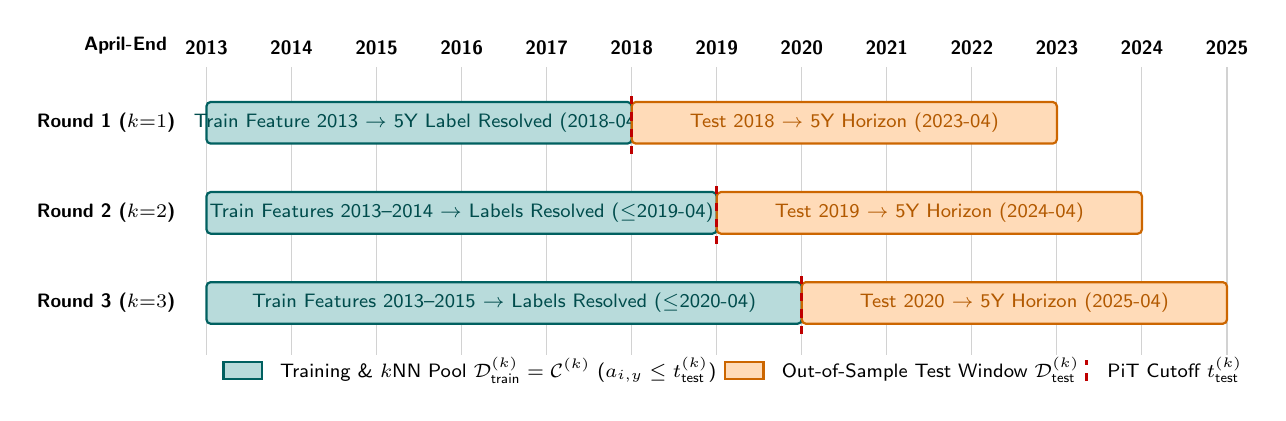
\begin{tikzpicture}[
    font=\sffamily\footnotesize,
    xscale=1.08, yscale=0.88
]

% Year axis header (2013 to 2025)
\foreach \yr/\x in {2013/0, 2014/1, 2015/2, 2016/3, 2017/4, 2018/5, 2019/6, 2020/7, 2021/8, 2022/9, 2023/10, 2024/11, 2025/12} {
    \draw[gray!35, thin] (\x, 0.2) -- (\x, 4.35);
    \node[font=\sffamily\scriptsize\bfseries, anchor=south] at (\x, 4.4) {\yr};
}
\node[font=\sffamily\scriptsize, anchor=south east] at (-0.35, 4.4) {\textbf{April-End}};

% Round 1 (y = 3.2..3.9): Train feature 2013 (5Y outcome ends 2018-04), Test feature 2018 (5Y ends 2023-04)
\node[anchor=east, font=\sffamily\scriptsize\bfseries] at (-0.25, 3.55) {Round 1 ($k{=}1$)};
\fill[teal!28, draw=teal!75!black, thick, rounded corners=1.5pt] (0, 3.25) rectangle (5, 3.85);
\node[font=\sffamily\scriptsize, text=teal!60!black] at (2.5, 3.55) {Train Feature 2013 $\rightarrow$ 5Y Label Resolved (2018-04)};
\fill[orange!28, draw=orange!80!black, thick, rounded corners=1.5pt] (5, 3.25) rectangle (10, 3.85);
\node[font=\sffamily\scriptsize, text=orange!70!black] at (7.5, 3.55) {Test 2018 $\rightarrow$ 5Y Horizon (2023-04)};
\draw[red!75!black, very thick, dashed] (5, 3.1) -- (5, 4.0);

% Round 2 (y = 1.9..2.6): Train features 2013-2014 (outcomes end <= 2019-04), Test feature 2019 (ends 2024-04)
\node[anchor=east, font=\sffamily\scriptsize\bfseries] at (-0.25, 2.25) {Round 2 ($k{=}2$)};
\fill[teal!28, draw=teal!75!black, thick, rounded corners=1.5pt] (0, 1.95) rectangle (6, 2.55);
\node[font=\sffamily\scriptsize, text=teal!60!black] at (3.0, 2.25) {Train Features 2013--2014 $\rightarrow$ Labels Resolved ($\le$2019-04)};
\fill[orange!28, draw=orange!80!black, thick, rounded corners=1.5pt] (6, 1.95) rectangle (11, 2.55);
\node[font=\sffamily\scriptsize, text=orange!70!black] at (8.5, 2.25) {Test 2019 $\rightarrow$ 5Y Horizon (2024-04)};
\draw[red!75!black, very thick, dashed] (6, 1.8) -- (6, 2.7);

% Round 3 (y = 0.6..1.3): Train features 2013-2015 (outcomes end <= 2020-04), Test feature 2020 (ends 2025-04)
\node[anchor=east, font=\sffamily\scriptsize\bfseries] at (-0.25, 0.95) {Round 3 ($k{=}3$)};
\fill[teal!28, draw=teal!75!black, thick, rounded corners=1.5pt] (0, 0.65) rectangle (7, 1.25);
\node[font=\sffamily\scriptsize, text=teal!60!black] at (3.5, 0.95) {Train Features 2013--2015 $\rightarrow$ Labels Resolved ($\le$2020-04)};
\fill[orange!28, draw=orange!80!black, thick, rounded corners=1.5pt] (7, 0.65) rectangle (12, 1.25);
\node[font=\sffamily\scriptsize, text=orange!70!black] at (9.5, 0.95) {Test 2020 $\rightarrow$ 5Y Horizon (2025-04)};
\draw[red!75!black, very thick, dashed] (7, 0.5) -- (7, 1.4);

% Legend at bottom
\fill[teal!28, draw=teal!75!black, thick] (0.2, -0.15) rectangle (0.65, 0.1);
\node[anchor=west, font=\sffamily\scriptsize] at (0.75, -0.02) {Training \& $k$NN Pool $\mathcal{D}_{\text{train}}^{(k)} = \mathcal{C}^{(k)}$ ($a_{i,y} \le t_{\text{test}}^{(k)}$)};

\fill[orange!28, draw=orange!80!black, thick] (6.1, -0.15) rectangle (6.55, 0.1);
\node[anchor=west, font=\sffamily\scriptsize] at (6.65, -0.02) {Out-of-Sample Test Window $\mathcal{D}_{\text{test}}^{(k)}$};

\draw[red!75!black, very thick, dashed] (10.35, -0.18) -- (10.35, 0.13);
\node[anchor=west, font=\sffamily\scriptsize] at (10.48, -0.02) {PiT Cutoff $t_{\text{test}}^{(k)}$};

\end{tikzpicture}
}
\caption{Three-round non-overlapping walk-forward split across 2013--2020 April-end windows. The red dashed barrier $t_{\text{test}}^{(k)}$ enforces $a_{i,y} = t_y + 5\text{Y} \le t_{\text{test}}^{(k)}$ so that neither LightGBM training nor $k$NN case retrieval observes unresolved five-year outcomes.}
\label{fig:walkforward}
\end{figure*}

Table~\ref{tab:experiments} defines the quantitative validation criteria for Experiments E1--E4 (plus E5 sensitivity analyses on 5-day and 60-day terminal windows and single-factor screens such as low P/B and high ROE). All E1--E5 benchmarks remain \emph{pending hypotheses} to be empirically tested upon completion of \texttt{build\_dataset.py}, \texttt{train.py}, \texttt{evaluate.py}, and \texttt{agent.py}.

% [6.2] Quantitative Validation Targets Table (E1-E4)
\begin{table*}[t]
\centering
\caption{Planned Evaluation Protocol and Quantitative Validation Criteria (Experiments E1--E4; Pending Execution)}
\label{tab:experiments}
\renewcommand{\arraystretch}{1.14}
\scriptsize
\begin{tabularx}{\textwidth}{L{2.25cm} L{3.35cm} L{3.45cm} Y}
\toprule
\textbf{Experiment} & \textbf{Core Evaluation Metrics} & \textbf{Comparison Baselines} & \textbf{Quantitative Validation Criterion (Pending Hypothesis)} \\
\midrule
\textbf{E1: Ranking Quality} (RQ1) &
Per-round \texttt{Precision@20}, \texttt{Precision@50}, \texttt{Recall@50}, \texttt{PR-AUC} &
In-round actual positive rate ($\le 5\%$) and 1,000 fixed-seed Monte Carlo random draws; Logistic Regression; single-factor rules &
Test whether LightGBM \texttt{Precision@50} and \texttt{PR-AUC} exceed the in-round actual positive rate and surpass the 95th percentile of 1,000 random draws \\
\midrule
\textbf{E2: Portfolio Behavior} (RQ1) &
Equal-weighted top-50 5-year cumulative adjusted gross return, Maximum Drawdown (MDD) &
TWSE 0050 ETF adjusted total return over identical entry ($t + 1$ trading day close) and 5-year holding horizon &
Assess whether top-50 equal-weighted gross returns and drawdown profile outperform 0050 across all three rounds (explicitly noting exclusion of fees/taxes) \\
\midrule
\textbf{E3: Feature Association} (RQ2) &
Stratified feature medians (\texttt{y\_main}$=1$, \texttt{y\_raw}$=1$ only, \texttt{y\_raw}$=0$, delisted) and cross-round SHAP rank correlation &
Full evaluable universe base rate and Yartseva \cite{yartseva2025} directional expectations &
Evaluate cross-window SHAP stability and whether features distinguish fundamental winners (\texttt{y\_main}$=1$) from multiple-expansion-only stocks (correlation only, not causality) \\
\midrule
\textbf{E4: Agent Report Reliability} (RQ3) &
Numerical accuracy, evidence citation rate, and required-field coverage across 30 sampled stocks &
Direct LLM prompting (same model version and raw \texttt{as-of} data, without whitelisted tools or \texttt{verify\_report}) &
Verify that 3-round \texttt{verify\_report} + \texttt{template\_report($T$)} achieves \textbf{100\% tool-number accuracy (zero fabricated values)} and superior field coverage over direct LLM \\
\bottomrule
\end{tabularx}
\end{table*}

\subsection{Key Limitations and Research Ethics}
Six structural limitations bound our interpretation: (1) early delisted companies in FinMind may lack historical financial statement records, leaving residual selection effects in \texttt{UNKNOWN}; (2) fixing annual reports at April-end introduces up to 16 months of feature lag; (3) excluding \texttt{UNKNOWN} instances from primary training improves label purity at the cost of reduced coverage; (4) E2 evaluates gross returns excluding brokerage commissions, securities transaction tax, and slippage; (5) uncalibrated model scores measure relative cross-sectional ranking rather than calibrated win probabilities; and (6) test windows (2018--2020) span trade-war and COVID-19 regimes prior to Taiwan's 2023--2026 AI hardware super-cycle (including sharp concentration drawdowns such as the November~2026 single-day plunge \cite{twse2026}). \emph{Disclaimer}: Multibagger Scout is designed strictly for academic research and financial education and does not constitute investment advice.

% =========================================================================
% SECTION V: CONCLUSION & FUTURE WORK (A-Z SOP: W, X, Y, Z)
% =========================================================================
\section{Conclusion and Future Work}

% [W. What Proposed]
Motivated by extreme long-term equity wealth concentration \cite{bessembinder2023, bessembinder2026} and the compound risks of look-ahead/survivorship bias \cite{gao2026}, black-box ML opacity \cite{gu2020}, LLM temporal leakage \cite{he2025chrono, didisheim2025}, and multi-variable arithmetic hallucinations \cite{faith2025, alphaarena2026}, this paper presented \textbf{Multibagger Scout}---a point-in-time, evidence-verifiable Domain AI Agent for five-year TWSE common stock ranking and analysis. Grounded in Program of Thoughts \cite{chen2023pot, agenticrag2026}, the system isolates all numerical feature engineering, LightGBM ranking, SHAP attribution, temporally resolved $k$NN retrieval ($\tau \le t - 5\text{Y}$), and two domain red-flag checks inside seven whitelisted deterministic tools, audited by a three-round \texttt{verify\_report} loop with deterministic template fallback.

% [X. eXcel]
The architecture offers two distinct advantages: (i) rigorous chronological and wealth-conservation hygiene across dividends, capital reductions, splits, delisted firms, and Emerging Board transitions; and (ii) auditable, zero-unauthorized-number financial explanations suitable for both individual fundamental research and financial AI pedagogy.

% [Y. Yields]
Completed data-stage validation demonstrates end-to-end engineering feasibility: 1,322 TWSE common stocks (including 93 delisted firms) were collected across 9,256 FinMind tasks with a 0\% failure rate; 7,754 clean firm-year observations (1,094 firms, 2013--2020) were built after excluding 394 Emerging Board observations; price anomalies fell from 14.7\% to 1.7\% (134 observations); external TSMC verification achieved 8/8 consistency; and capital-reduction wealth conservation was confirmed on stock 8201 (NT\$8,690) and 214/214 TWSE records.

% [Z. Zen & Future Work]
Immediate next steps execute the full formal dataset builder (\texttt{build\_dataset.py}), three-round walk-forward training (\texttt{train.py}), and E1--E5 evaluations (\texttt{evaluate.py}, \texttt{agent.py}). Future extensions beyond the core scope include backfilling early delisted financial statements, integrating quarterly filings and current-year monthly revenues to shorten feature lag, incorporating Market Observation Post System (MOPS) material announcements and advanced rules (such as asset growth exceeding EBITDA growth \cite{yartseva2025}), and adding transaction-cost modeling alongside post-hoc probability calibration.

\bibliographystyle{IEEEtran}
\bibliography{references}

\end{document}
